\documentclass{article}
\usepackage{amsmath}
\usepackage{amssymb}
\usepackage{mathtools}
\usepackage{fullpage}
\usepackage[T1]{fontenc}
\usepackage{lmodern}
\usepackage{tikz}
\usetikzlibrary{calc,intersections,through,backgrounds}
\usetikzlibrary{bayesnet}
\usepackage{tikzscale}
\usepackage{tkz-euclide}
\usepackage{tcolorbox}
\tcbuselibrary{skins,breakable}
% pgfplots
\usepackage{pgfplots}
\pgfplotsset{compat=1.8}
% For entities in text
\newcommand{\entity}[1]{\texttt{#1}}
% For entities in pgfplots
\newcommand{\entpgf}[1]{\texttt{#1}}

\begin{document}
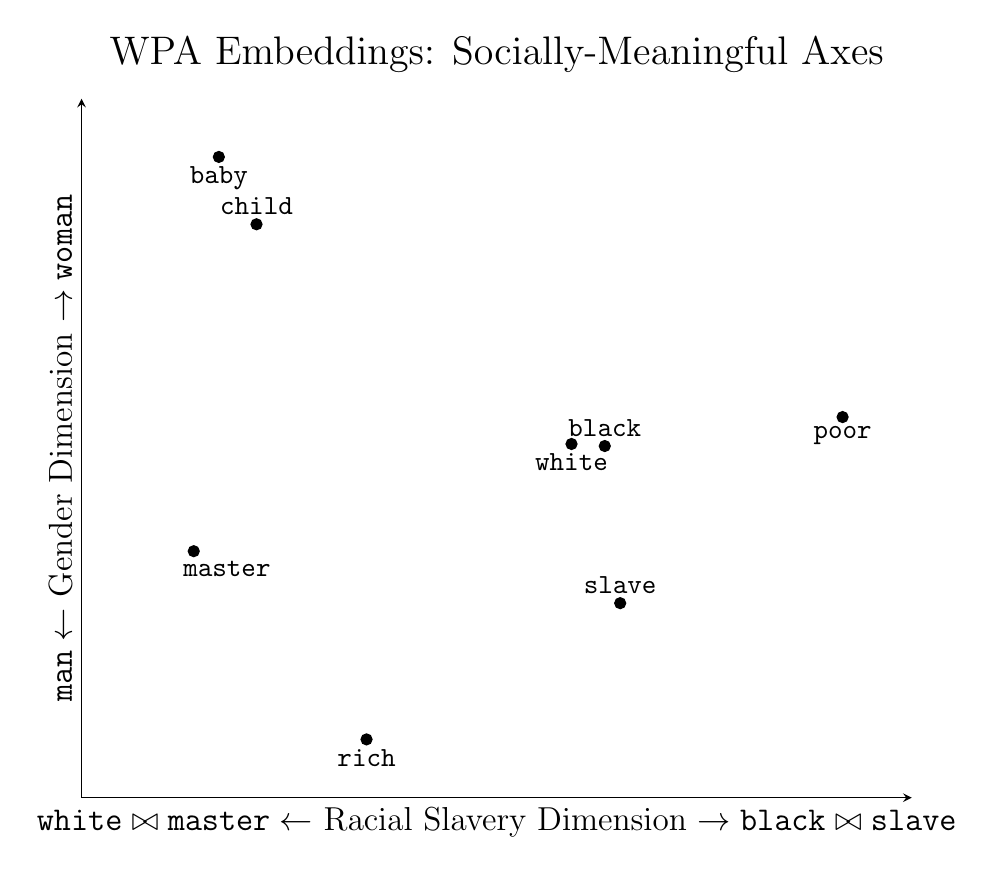
\begin{tikzpicture}
\pgfplotsset{ticks=none}
		\begin{axis}[
			title={\Large WPA Embeddings: Socially-Meaningful Axes},
			separate axis lines,
		    axis x line=bottom,
			axis y line=left,
			xmin=-1.0687146-0.3009931564331055, xmax=1.941217+0.3009931564331055,
			ymin=-1.0480828-0.21689443588256838, ymax=1.1208615+0.21689443588256838,
			xtick={-1.0687146,1.941217},ytick={-1.0480828,1.1208615},
			xlabel={\large $\entity{white} \bowtie \entity{master} \leftarrow$ Racial Slavery Dimension $\rightarrow \entity{black} \bowtie \entity{slave}$},ylabel={\large $\entity{man} \leftarrow$ Gender Dimension $\rightarrow \entity{woman}$},
			%x label style={anchor=west},
			%y label style={anchor=south},
			width=\textwidth
			]
			\addplot+[mark options={fill=black,color=black},only marks,point meta=explicit symbolic, nodes near coords] coordinates {
%(-0.9854497909545898, -0.42804527282714844)[]
%(-1.0687146186828613, 0.5719547271728516)[]
(-0.8816595077514648, -0.3472309112548828)[]
(0.9065628051757812, 0.04435586929321289)[]
(0.9736499786376953, -0.5407805442810059)[]
(0.7618718147277832, 0.05193376541137695)[]
(-0.6085567474365234, 0.8700709342956543)[]
(-0.7724103927612305, 1.120861530303955)[]
(1.9412169456481934, 0.1522383689880371)[]
(-0.12992000579833984, -1.0480828285217285)[]
%(-0.05989360809326172, -0.14764881134033203)[]
%(0.9401063919067383, -0.24821233749389648)[]

};
\node (master) at (axis cs:-0.8816595077514648, -0.3472309112548828){};
\node (black) at (axis cs:0.9065628051757812, 0.04435586929321289){};
\node (slave) at (axis cs:0.9736499786376953, -0.5407805442810059){};
\node (white) at (axis cs:0.7618718147277832, 0.05193376541137695){};
\node (child) at (axis cs:-0.6085567474365234, 0.8700709342956543){};
\node (baby) at (axis cs:-0.7724103927612305, 1.120861530303955){};
\node (poor) at (axis cs:1.9412169456481934, 0.1522383689880371){};
\node (rich) at (axis cs:-0.12992000579833984, -1.0480828285217285){};
\node (whitemaster) at (axis cs:-0.05989360809326172, -0.14764881134033203){};
\node (blackslave) at (axis cs:0.9401063919067383, -0.24821233749389648){};
\node [inner sep=0] (intersect) at (axis cs:-1.0168094635009766, -0.05141639709472656){};
\node[anchor = north, xshift=12.0, yshift=0.0] (masterl) at(axis cs: -0.8816595077514648, -0.3472309112548828){$\entpgf{master}$};
\node[anchor = south, xshift=0.0, yshift=0.0] (blackl) at(axis cs: 0.9065628051757812, 0.04435586929321289){$\entpgf{black}$};
\node[anchor = south, xshift=0.0, yshift=0.0] (slavel) at(axis cs: 0.9736499786376953, -0.5407805442810059){$\entpgf{slave}$};
\node[anchor = north, xshift=0.0, yshift=0.0] (whitel) at(axis cs: 0.7618718147277832, 0.05193376541137695){$\entpgf{white}$};
\node[anchor = south, xshift=0.0, yshift=0.0] (childl) at(axis cs: -0.6085567474365234, 0.8700709342956543){$\entpgf{child}$};
\node[anchor = north, xshift=0.0, yshift=0.0] (babyl) at(axis cs: -0.7724103927612305, 1.120861530303955){$\entpgf{baby}$};
\node[anchor = north, xshift=0.0, yshift=0.0] (poorl) at(axis cs: 1.9412169456481934, 0.1522383689880371){$\entpgf{poor}$};
\node[anchor = north, xshift=0.0, yshift=0.0] (richl) at(axis cs: -0.12992000579833984, -1.0480828285217285){$\entpgf{rich}$};

%\draw[ultra thin] (axis cs:\pgfkeysvalueof{/pgfplots/xmin},0) -- (axis cs:\pgfkeysvalueof{/pgfplots/xmax},0);
%\draw[ultra thin] (axis cs:0,\pgfkeysvalueof{/pgfplots/ymin}) -- (axis cs:0,\pgfkeysvalueof{/pgfplots/ymax});

\end{axis}
\end{tikzpicture}
\end{document}
